\chapter{Implementation, Related Work and Evaluation}\label{ch:evaluation}

\section{Pilot Implementation}\label{sec:implementation}
% Все предложенные в данной работе подходы реализованы в созданном в рамках данной работы Хорн-решателе \theringen{} (\emph{R}egular \emph{In}variant \emph{Gen}erator)\footnote{\url{https://github.com/Columpio/RInGen}}.
% Реализация занимает 5200 строк на языке \fsharp{}.
% Было принято решение реализовать Хорн-решатель с нуля, не встраиваясь в кодовые базы существующих решателей, поскольку предложенные алгоритмы требуют нетривиальных манипуляций с формулами и результатами других логических решателей.
All the approaches proposed in this work are implemented in a Horn solver \theringen{} (\emph{R}egular \emph{In}variant \emph{Gen}erator)\footnote{\url{https://github.com/Columpio/RInGen}}.
The implementation comprises 5200 lines of \fsharp{} code. A Horn solver is developed from scratch as proposed algorithms require non-trivial manipulations of formulas and the results of other logical solvers.

% Общая архитектура реализованного инструмента представлена на рисунке~\ref{fig:ringen-arch}.
% Инструмент \theringen{} принимает на вход систему дизъюнктов Хорна с ограничениями в формате SMTLIB2~\cite{BarFT-RR-17}.
% После парсинга дизъюнктов выполняется их упрощение, в частности, устранение равенств, селекторов и тестеров. Затем, в зависимости от поданных Хорн-решателю опций, запускается один из алгоритмов, предложенных в данной работе. Результатом работы каждого из них является формула над неинтерпретированными функциями, которая передаётся в сторонний логический решатель~--- \vampire{} или \cvc{}.
% В итоге инструмент возвращает безопасный индуктивный инвариант, если система безопасна, в противном случае~--- резолютивное опровержение.
The overall architecture of the tool is presented in Figure~\ref{fig:ringen-arch}.
\theringen{} takes as input a CHC system in the SMTLIB2 format~\cite{BarFT-RR-17}.
The CHC system is parsed and simplified: equalities, selectors, and testers are eliminated. Then, depending on the options submitted to the solver, one of the algorithms proposed in this work is started.
A ``Substitution of ADT with uninterpreted functions module'' implements the algorithm from the Chapter~\ref{ch:fmf}, and the ``Tree automata first-order declaration generator'' implements the algorithm from the Chapter~\ref{ch:SyncReg}.
The output of each of these algorithms is a formula over uninterpreted functions. It is passed to an external logical solver~--- either \vampire{} automated theorem prover or \cvc{} SMT-solver.
As a result, \theringen{} returns a safe inductive invariant if the CHC system is satisfiable, otherwise, it returns a resolution refutation.

\begin{figure}[h]
% https://online.visual-paradigm.com/share.jsp?id=323637353533352d31
    \centering
    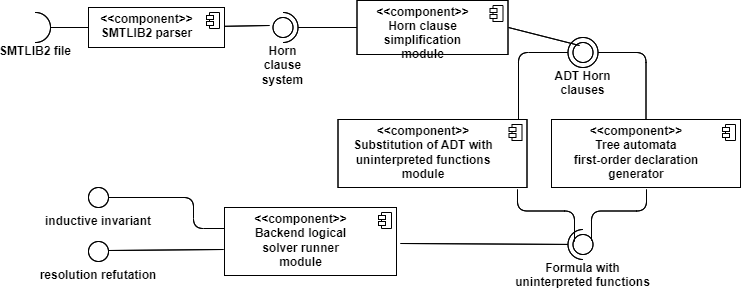
\includegraphics[width=\textwidth]{Dissertation/images/arch.png}
    \caption{Architecture of \theringen{}}
    \label{fig:ringen-arch}
\end{figure}

\textbf{\theringen{}.}\label{sec:ringen-pure}
% Итак, подход, представленный в главе~\ref{ch:fmf}, реализован автором данного исследования в рамках Хорн-решателя \theringen{}.
% Как сам подход, так и его реализация подразумевают использование стороннего SMT-решателя $\verifier$ для теории неинтерпретированных функций с кванторами, поэтому предлагаемая реализация в дальнейшем будет обозначаться $\ringen{\verifier}$.
% В частности, в качестве решателя $\verifier$ в экспериментах используются инструмент \vampire{}~\cite{reger2017instantiation} и SMT-решатель \cvc{}.
% Инструмент \vampire{} использует портфолио- подход~\cite{reger2014challenges}, то есть перебирает различные техники проверки выполнимости формул, построенные на насыщении системы~\cite{kovacs2013first} или на поиске конечных моделей~\cite{10.1007/978-3-319-40970-2_20}.
% Инструмент \cvc{} используется в режиме построения конечных моделей\footnote{с опцией \texttt{-{}-finite-model-find}}~\cite{reynolds2013finite}.
% Оба инструмента позволяют как доказывать безопасность системы, так и находить контрпримеры.
That is, we implemented the approach presented in Chapter~\ref{ch:fmf} within the \theringen{} Horn solver. 
Both the approach itself and its implementation involve the use of an external solver $\verifier$ for the theory of uninterpreted functions with quantifiers, therefore the proposed implementation will be further denoted as $\ringen{\verifier}$.
Specifically, \vampire{}~\cite{reger2017instantiation} and the SMT solver \cvc{} are used as the $\verifier$ in the experiments.
\vampire{} uses a portfolio-based approach~\cite{reger2014challenges}: it iterates through various satisfiability checking techniques, mostly based on saturation of the system~\cite{kovacs2013first} and finite model finding~\cite{10.1007/978-3-319-40970-2_20}.
\cvc{} is used in the finite model finding mode\footnote{with the \texttt{-{}-finite-model-find} option}~\cite{reynolds2013finite}.
Both tools can prove the satisfiability of the system and finding counterexamples.

\textbf{\ringenSync{}.}
% Этот подход представленный в главе~\ref{ch:SyncReg}, реализован как надстройка над $\ringen{\verifier}$.
% В качестве стороннего решателя $\verifier$ в экспериментах использовался \cvc{}, поскольку \ringenSync{} порождает символы с большой арностью, которые не поддерживаются инструментом \vampire{}\footnote{\url{https://github.com/vprover/vampire/issues/348\#issuecomment-1091782513}}.
% Эта реализация в дальнейшем будет обозначаться \ringenSync{}\footnote{\url{https://github.com/Columpio/RInGen/releases/tag/ringen-tta}}.
The approach presented in Chapter~\ref{ch:SyncReg} is implemented as an extension of $\ringen{\verifier}$.
In the experiments, \cvc{} is used as the external solver $\verifier$, as \ringenSync{} generates symbols with high arity, which are not supported by \vampire{}\footnote{\url{https://github.com/vprover/vampire/issues/348\#issuecomment-1091782513}}.
Thus, the implementation will be hereinafter referred to as \ringenSync{}\footnote{\url{https://github.com/Columpio/RInGen/releases/tag/ringen-tta}}.

\textbf{\theringenCICI{}.}
% Данный подход, представленный в главе~\ref{ch:cici}, реализован в рамках кодовой базы Хорн-решателей \racer{}~\cite{10.1145/3498722} (развитие Хорн-решателя \spacer{}~\cite{komuravelli2016smt}, реализованное в логическом решателе \zprover{}\footnote{\url{https://github.com/Columpio/z3/tree/racer-solver-interaction}}) и Хорн-решателя $\ringen{\verifier{}}$\footnote{\url{https://github.com/Columpio/RInGen/releases/tag/chccomp22}}, описанного выше.
% Эта реализация в дальнейшем будет обозначаться $\ringenCICI{\verifier{}}$. Далее описаны обе части этой реализации в Хорн-решателях \racer{} и $\ringen{\verifier{}}$, соответственно, которые далее называются \emph{базовыми} относительно инструмента $\ringenCICI{\verifier{}}$.
The approach presented in Chapter~\ref{ch:cici} is implemented within the codebase of the Horn solvers \racer{}~\cite{10.1145/3498722} (a successor of the \spacer{} Horn solver~\cite{komuravelli2016smt}, implemented in the logical solver \zprover{}\footnote{\url{https://github.com/Columpio/z3/tree/racer-solver-interaction}}) and the Horn solver $\ringen{\verifier{}}$\footnote{\url{https://github.com/Columpio/RInGen/releases/tag/chccomp22}}.
This implementation will be referred to as $\ringenCICI{\verifier{}}$. Both parts of this implementation in the Horn solvers \racer{} and $\ringen{\verifier{}}$ are described below. These Horn solvers will be referred to as \emph{basic} with respect to the $\ringenCICI{\verifier{}}$ Horn solver.

% Хорн-решатель \racer{} разработан Ари Гурфинкелем (Arie Gurfinkel) и Хари Говинд Ведирамана Кришнаном (Hari Govind Vediramana Krishnan) из университета Ватерлоо.
% Инструмент \racer{} основан на подходе, называемом достижимость, направляемая свойством (Property-Directed Reachability, PDR)~\cite{komuravelli2016smt}, который можно рассматривать как сложный экземпляр \cegar{}.
% PDR строит абстрактные состояния в виде конъюнкции формул (называемых \emph{леммами}) на различных \emph{уровнях} путём итеративного увеличения уровня в цикле.
% При этом поддерживаются следующие возможности: если набор лемм $\{\phi_i\}$ был построен на уровне $n$, то $\bigwedge_i \phi_i$ аппроксимирует сверху все состояния, достижимые менее чем за $n$ шагов перехода, и аппроксимирует снизу свойство безопасности.
% Таким образом, леммы в PDR выполняют требование абстракции в процедуре \RunBlackBox{} (алгоритм~\ref{code:runblackbox}).
% Хорн-решатель \racer{} был модифицирован в рамках данного диссертационного исследования таким образом, чтобы в конце каждой итерации набор лемм последнего уровня асинхронно передавался новому процессу инструмента $\ringen{\verifier{}}$.
The \racer{} Horn solver is developed by Arie Gurfinkel and Hari Govind Vediramana Krishnan from the University of Waterloo. It is based on an approach called Property-Directed Reachability (PDR)~\cite{komuravelli2016smt}, which can be viewed as a complex instance of \cegar{}. PDR builds abstract states in the form of conjunctions of formulas (called \emph{lemmas}) at various \emph{levels} by iteratively increasing the level in a loop. The following properties of lemma sets are maintained: if a set of lemmas $\{\phi_i\}$ is constructed at level $n$, then $\bigwedge_i \phi_i$ over-approximates all states reachable in less than $n$ transition steps, and under-approximates the safety property. Thus, PDR lemmas fulfill the requirement of abstraction in the \RunBlackBox{} procedure (see Listing~\ref{code:runblackbox}). \racer{} is modified to asynchronously pass the set of lemmas from the last level to a new process of $\ringen{\verifier{}}$ at the end of each iteration.

% Процедура \RunBlackBox{} (алгоритм~\ref{code:runblackbox}) реализована на основе инструмента  $\ringen{\verifier{}}$. Было выполнено следующее обобщение в процедуре $\substituteLemmas(\prog, a)$ (см.~\autoref{sec:subst_lemmas}).
% Конъюнктивная форма лемм инструмента \racer{} используется для вывода инвариантов более общего вида:
% $\bigwedge_i(\phi_i(\overline{x})\,\lor\,\overline{x}\!\in\!L_i)$.
% Так, имея $a(P) = \bigwedge_i \phi_i$,
% мы заменяем все атомы $P(\overline{t})$ на \emph{конъюнкцию дизъюнкций} $\bigwedge_i (\phi_i(\overline{t})\lor L_i(\overline{t}))$ с новыми предикатными символами $L_i$.
% Это позволяет выводить более общие инварианты, чем инварианты из объединения классов $\elemclass{}$ и $\abstrDomain$ (см. определение~\ref{def:combined-class}), которое состоит только из формул вида $\phi(\overline{x})\,\lor\,\overline{x}\!\in\!L$.
The \RunBlackBox{} procedure (see Listing~\ref{code:runblackbox}) is implemented in the $\ringen{\verifier{}}$. The following generalization of the $\substituteLemmas(\prog, a)$ procedure (see~\autoref{sec:subst_lemmas}) is implemented. The conjunctive form of lemmas from \racer{} is used to infer invariants with a more general shape: $\bigwedge_i(\phi_i(\overline{x})\,\lor\,\overline{x}\!\in\!L_i)$. Hence, given $a(P) = \bigwedge_i \phi_i$, we replace all atoms $P(\overline{t})$ with a \emph{conjunction of disjunctions} $\bigwedge_i (\phi_i(\overline{t})\lor L_i(\overline{t}))$ with new predicate symbols $L_i$. This allows inferring more general invariants than those from the union of $\elemclass{}$ and $\abstrDomain$ (see Definition~\ref{def:combined-class}), which consists only of formulas of the form $\phi(\overline{x})\,\lor\,\overline{x}\!\in\!L$.

% После преобразований модифицированный $\ringen{\verifier{}}$ вызывает сторонний решатель $\verifier{}$ с ограничением по времени в 30 секунд.
% Затем его результаты передаются обратно в Хорн-решатель \racer{}, где они асинхронно обрабатываются.
% Кроме того, реализация не выполняет дорогостоящее преобразование в КНФ из алгоритма~\ref{code:residual-chc}, так как реализация $\ringen{\verifier{}}$ позволяет принимать на вход дизъюнкты Хорна в произвольном виде, поскольку он полагается на сторонний решатель $\verifier{}$ с полной поддержкой логики первого порядка.
After the transformations, the $\ringen{\verifier{}}$ calls the external solver $\verifier{}$ with a 30 second time limit. Then its results are passed back to \racer{}, where they are processed asynchronously. Moreover, the implementation does not perform the costly CNF transformation from Listing~\ref{code:residual-chc}, as the $\ringen{\verifier{}}$ takes Horn clauses in arbitrary form, since it relies on the external solver $\verifier{}$ with full first-order logic support.

\section{Related Work}\label{ch:relatedWork}

% Раздел~\cref{sec:relatedWork/hornSolvers} данной главы посвящен сравнению предложенных методов решения систем дизъюнктов Хорна с алгебраическими типами данных и существующих методов, реализованных в таких инструментах, как \spacer{}, \racer{}, \eldarica{}, \vericat{}, \hoice{} и \rchc{}. Данные инструменты были отобраны по следующему принципу: инструменты, поддерживающие системы дизъюнктов Хорна над алгебраическими типами данных, которые проверяют как выполнимость, так и не выполнимость этих систем. Так, например, не рассматривались инструменты, решающие родственную проблему автоматизации индукции для теорем с алгебраическими типами данных, такие как, например, \cvc{} в режиме индукции~\cite{reynolds2015induction} (см. предыдущий раздел), \textsc{AdtInd}~\cite{10.1007/978-3-030-30048-7_35} и пр., поскольку они не принимают на вход системы дизъюнктов Хорна. Также не рассматривались инструменты логического программирование (такие, как \textsc{Prolog}~\cite{ClocksinMellish03}), поскольку они позволяют проверять только невыполнимость систем дизъюнктов Хорна и ничего не говорят об их выполнимости.
This section is dedicated to the comparison of proposed methods for solving Horn clause systems with algebraic data types and existing methods, implemented in tools such as \spacer{}, \racer{}, \eldarica{}, \vericat{}, \hoice{}, and \rchc{}. We selected only the tools supporting Horn clause systems over algebraic data types that verify both the satisfiability and unsatisfiability of these systems. For instance, tools addressing the related problem of automating induction for theorems with algebraic data types, such as, for example, \cvc{} in induction mode~\cite{reynolds2015induction}, \textsc{AdtInd}~\cite{10.1007/978-3-030-30048-7_35} and others are not considered, as they do not accept Horn clause systems as input. Also, logic programming tools (such as \textsc{Prolog}~\cite{ClocksinMellish03}) are not considered because they only check the unsatisfiability of Horn clause systems and cannot show their satisfiability.

\begin{table} [htbp]
    \centering\small
    \begin{threeparttable}% выравнивание подписи по границам таблицы
        \caption{Comparison of Horn solvers with ADT support}\label{tab:hornSolvers}%
        \begin{tabular}{| m{50mm} || x{25mm} | x{25mm} | x{25mm} | x{25mm} |}
            \hline
            \hline
Tool & Invariant class & Method & Returns the invariant & Fully automatic\\\hline\hline
\spacer{} & \elemclass{} & \pdr{} & Yes & Yes\\
\racer{} & \catelemclass{} & \pdr{} & No & No\\
\eldarica{} & \sizeelemclass{} & \cegar{} & Yes & Yes\\
\vericat{} & -- & Transf. & No & Yes\\
\hoice{} & \elemclass{} & \ice{} & Yes & Yes\\
\rchc{}  & \syncRegFlatClass{} & \ice{} & Yes & Yes\\\hline
\ringen{\cvc} & \regclass{} & Transf. + \fmf{} & Yes & Yes\\
\ringen{\vampire} & -- & Transf. + \satur{} & No & Yes\\
\ringenSync{} & \syncRegFullClass{} & Transf. + \fmf{} & Yes & Yes\\
\ringenCICI{\cvc} & \regelemclass{} & \ourCEGAR{} & Yes & Yes\\
\ringenCICI{\vampire} & -- & \ourCEGAR{} & No & Yes\\
            \hline
            \hline
        \end{tabular}
    \end{threeparttable}
\end{table}

% В таблице~\cref{tab:hornSolvers} представлены результаты сравнения работе Хорн-решателей~--- существующих (верхний блок) и предложенных в данной (нижний блок). Предложенные Хорн-решатели описаны в предыдущей главе~\ref{ch:evaluation}, реализуемые ими методы описаны в главах~\ref{ch:fmf},~\ref{ch:SyncReg} и~\ref{ch:cici} данной работы. В таблице, для краткости, название \theringen{} сокращено до \theringen{}, так, например, Хорн-решатель \ringenSync{} в таблице представлен как \ringenSync{}. Под словом <<Transf.>> имеется в виду, что инструмент построен на применении нетривиальных трансформаций к системе; аббревиатура <<FMF>> обозначает применение автоматического поиска конечных моделей (<<finite-model finding>>, см., например,~\cite{10.1007/978-3-319-40970-2_20,reynolds2013finite}); прочерк в столбце <<Класс инвариантов>> означает следующее: несмотря на то, что при выполнимости системы вывод инструмента неявно кодирует её индуктивный инвариант, не существует всюду останавливающейся процедуры, позволяющей этот вывод проверить. Остальные обозначения поясняются в подразделах, посвящённых соответствующим инструментам.
Table~\cref{tab:hornSolvers} presents the comparison of Horn solvers: existing ones (upper block) and those proposed in this work (lower block). The proposed Horn solvers are described in previous Section~\ref{sec:implementation}, and the methods they implement are described in Chapters~\ref{ch:fmf},~\ref{ch:SyncReg}, and~\ref{ch:cici} of this work. The word ``Transf.'' indicates that the tool is built using non-trivial transformations of the system; ``\fmf{}'' denotes the application of automatic finite-model finding (e.\:g., see~\cite{10.1007/978-3-319-40970-2_20,reynolds2013finite}); a dash in the ``Invariant class'' column means the following: although the output of the tool implicitly encodes its inductive invariant when the system is satisfiable, there is no always halting procedure that can check this output. The other designations are explained in the subsections dedicated to corresponding tools.

% Большинство рассмотренных инструментов отличаются классами, в которых они ищут индуктивные инварианты. Сравнение самих классов инвариантов было приведено в главе~\cref{ch:comparison}. В контексте сопоставления инструментов сравнение их классов инвариантов важно по следующей причине: если инструмент выводит инварианты в некотором классе, то проблема невыразительности этого класса (невозможность выразить определённые типы отношений) превращается в проблему незавершаемости этого инструмента. Иными словами, поскольку ни один из существующих инструментов не проверяет, существует ли \emph{вообще} инвариант для данной системы дизъюнктов Хорна в его классе\footnote{С одной стороны, эта задача по сложности сравнима с самой задачей верификации, с другой же стороны до сих пор ей были посвящены лишь отдельные работы (см., например,~\cite{10.1145/3022187,10.1145/2837614.2837640})}, то в случае отсутствия такового инструмент не будет завершаться.
Inductive invariant classes of most of the examined tools differ. A comparison of these invariants classes is given in Chapter~\cref{ch:comparison}. It is important for comparing tools because if a tool infers invariants in a certain class, then the expressiveness problem of this class (the inability to express certain types of relations) becomes the problem of non-termination of this tool. In other words, since none of the existing tools checks whether for a given Horn clause system there is an invariant in its class \emph{at all}\footnote{On the one hand, this task is as complex as the verification task itself; on the other hand, so far only a few studies have been dedicated to it (see, for example,~\cite{10.1145/3022187,10.1145/2837614.2837640})}, then the tool will not terminate in case of the absence of the invariant.

% Далее приведено краткое сравнительное описание существующих инструментов.
Further on, we provide a comparative description of the existing tools.

% \paragraph{Инструмент \spacer{}~\cite{komuravelli2016smt}} строит элементарные модели (класс \elemclass{} из раздела~\cref{sec:elem-def}). Этот инструмент создан на основе классической разрешающей процедуры для АТД, а также процедуры интерполяции и устранения кванторов~\cite{bjorner2015playing}. Ядром инструмента является подход \spacer{}, который основан на технике, называемой \emph{достижимость, направляемая свойством} \foreignlanguage{english}{(property-directed reachability, \pdr{})}, которая равномерно распределяет время анализа между поиском контрпримеров и построением безопасного индуктивного инварианта, распространяя информацию о достижимости небезопасных свойств и частичные леммы о безопасности. Инструмент позволяет выводить инварианты в комбинации алгебраических и других типов данных, возвращает проверяемые сертификаты. Подход, используемый в инструменте, корректен и полон. Недостатком инструмента является то, что он выражает инварианты в языке ограничений, а потому часто не завершается на проблемах с АТД.
\paragraph{The \spacer{} tool~\cite{komuravelli2016smt}} constructs elementary models (the \elemclass{} class). This tool is based on a classic satisfiability procedure for ADTs, as well as interpolation and quantifier elimination procedures~\cite{bjorner2015playing}. At its core, the tool employs a technique called \emph{property-directed reachability} (\pdr{}), which evenly distributes analysis time between counterexample search and safe inductive invariant inference, propagating information about reachability of unsafe properties and partial safety lemmas. The tool can infer invariants in a combination of algebraic and other data types, and returns verifiable certificates. The approach used in the tool is both sound and complete. A drawback of the tool is that it expresses invariants in the constraint language, and therefore often does not terminate on problems with ADTs.

% \paragraph{Инструмент \racer{}~\cite{10.1145/3498722}} является развитием инструмента \spacer{}, позволяя выводить инварианты в языке ограничений, расширенном катаморфизмами. Этот язык ограничений обозначен в таблице~\ref{tab:hornSolvers} как \catelemclass{}. \racer{} также наследует все достоинства подхода \spacer{}. Недостатком подхода является то, что он не полностью автоматический, поскольку требует вручную описывать катаморфизмы, что может быть затруднительно на практике, поскольку по заданной проблеме бывает сложно понять, какие катаморфизмы потребуются для её инварианта. Недостатком самого инструмента является то, что он не возвращает какие-либо проверяемые сертификаты с катаморфизмами.
\paragraph{The \racer{} tool~\cite{10.1145/3498722}} is an evolution of the \spacer{} tool. It can infer invariants in the constraint language extended with catamorphisms. This constraint language is denoted in the Table~\ref{tab:hornSolvers} as \catelemclass{}. \racer{} inherits all the advantages of the \spacer{} approach. A drawback of the approach is that it is not fully automatic, as it requires manually specifying catamorphisms, which can be challenging in practice because it can be hard to guess which catamorphisms will be required for the invariant of the given problem. A drawback of the tool is that it does not return any verifiable certificates.

% \paragraph{Инструмент \eldarica{}~\cite{8603013}} строит модели с ограничениями размера термов, которые вычисляют общее количество вхождений конструкторов (\sizeelemclass{} из раздела~\cref{sec:sizeelem-def}). Это расширение весьма ограниченно увеличивает выразительность языка ограничений, поскольку введённая функция считает количество всех конструкторов одновременно, поэтому с её помощью невозможно выразить многие свойства, например, ограничение на высоту дерева. Инструмент \eldarica{} использует подход \cegar{} с абстракцией предикатов и встроенный SMT-решатель \princess{}~\cite{princess}, который предоставляет разрешающую процедуру, а также процедуру интерполяции для АТД с ограничениями на размер термов. Эти процедуры построены на сведении данной теории к комбинации теорий неинтерпретируемых функций и линейной арифметики~\cite{hojjat2017deciding}.
\paragraph{The \eldarica{} tool~\cite{8603013}} constructs models with term size constraints, which calculate the total number of constructor occurrences (the \sizeelemclass{} class). This extension is very limited, as the introduced function counts all constructors at once, thus it cannot express many properties, such as properties depending on the tree height. The \eldarica{} tool employs the \cegar{} with predicate abstraction and an embedded SMT solver \princess{}~\cite{princess}, which provides a satisfiability and an interpolation procedures for algebraic data types with term size constraints. These procedures are based on the reduction of this theory to a combination of theories of uninterpreted functions and linear arithmetic~\cite{hojjat2017deciding}.

% \paragraph{Инструмент \vericat{}~\cite{10.1093/logcom/exab090,pettorossi_proietti_2022,10.1007/978-3-030-51074-9_6,angelis_fioravanti_pettorossi_proietti_2018}} обрабатывает условия проверки над теориями линейной арифметики и АТД и полностью устраняет АТД из исходной системы дизъюнктов путём сворачивания (fold), разворачивания (unfold), введения новых дизъюнктов и других трансформаций. После работы инструмента получается система дизъюнктов Хорна без АТД, на которой может быть запущен любой эффективный Хорн-решатель, например, \spacer{} или \eldarica{}. Основным достоинством подхода является тот факт, что он рассчитан на работу с проблемами, где алгебраические типы данных комбинированы с другими теориями. Основные недостатки подхода заключаются в следующем: сам процесс трансформации может также не завершаться, кроме этого из-за трансформации невозможно восстановить инвариант исходной системы, т.\:е. инструмент не возвращает проверяемого сертификата.
\paragraph{The \vericat{} tool~\cite{10.1093/logcom/exab090,pettorossi_proietti_2022,10.1007/978-3-030-51074-9_6,angelis_fioravanti_pettorossi_proietti_2018}} takes a CHC system over theories of linear arithmetic and ADTs and completely eliminates ADTs from the original system of Horn clauses by folding, unfolding, introducing new clauses, and other syntactic transformations. It produces a Horn clause system without ADTs, on which any efficient Horn solver, such as \spacer{} or \eldarica{}, can be run. The main advantage of this approach is that it is designed to work with problems where algebraic data types are combined with other theories. The main drawbacks of the approach are as follows: the transformation process itself may not terminate, and due to the transformation, it is impossible to recover the invariant of the original system, i.\:e., the tool does not return a verifiable certificate.

% \paragraph{Инструмент \hoice{}~\cite{10.1007/978-3-030-02768-1_8}} строит элементарные инварианты с помощью подхода, основанного на машинном обучении, \ice{}~\cite{10.1007/978-3-319-08867-9_5}. Его достоинством является возможность выводить инварианты в комбинации АТД с другими теориями, а также корректность и полнота, и, наконец, способность возвращать проверяемые сертификаты корректности. Его недостатком является то, что он выводит инварианты в невыразительном языке ограничений, а потому часто не завершается.
\paragraph{The \hoice{} tool~\cite{10.1007/978-3-030-02768-1_8}} constructs elementary invariants using a machine learning approach called \ice{}~\cite{10.1007/978-3-319-08867-9_5}. Its advantages include the ability to infer invariants for combinations of ADTs with other theories, as well as correctness and soundness, and finally, the ability to return verifiable correctness certificates. Its disadvantage is that it produces invariants in an inexpressive constraint language, and thus often does not terminate.

% \paragraph{Инструмент \rchc{}~\cite{haude2020,losekoot_et_al:LIPIcs.FSCD.2023.7},}также как и \hoice{}, использует подход \ice{}; \rchc{} основан на машинном обучении, однако выражает индуктивные инварианты программ над АТД при помощи \emph{автоматов над деревьями}~\cite{tata}. Но из-за сложностей с выражением кортежей термов автоматами, описанных в разделе~\ref{sec:comparison/undef-in-sync}, подход часто оказывается неприменим для простейших примеров, где существуют классические символьные инварианты. 
\paragraph{The \rchc{} tool~\cite{haude2020,losekoot_et_al:LIPIcs.FSCD.2023.7}} also uses the \ice{} approach; it expresses inductive invariants of programs over ADTs using \emph{tree automata}~\cite{tata}. However, due to the complexities of expressing tuples of terms with automata, described in Section~\ref{sec:comparison/undef-in-sync}, the approach is often inapplicable even for the simplest examples where classical symbolic invariants exist.

% \paragraph{Выводы.} Подводя итоги сравнения вышеозначенных инструментов и методов, можно сказать следующее. По сравнении с методом инструмента \rchc{} предложенные в данной диссертационной работе подходы являются альтернативными способами вывода регулярных инвариантов и их надклассов. Поэтому они могут быть совмещены с подходом инструмента \rchc{}, чтобы быстрее сходиться к индуктивному инварианту системы, если он существует. В сравнении с методами остальных существующих инструментов, предложенные подходы позволяют выводить инварианты в независимых классах регулярных инвариантов. Поэтому применение предложенных методов совместно с существующими позволит решать больше различных типов задач.
\paragraph{Conclusions.} Compared to the method of \rchc{}, the approaches proposed in this thesis provide alternative ways of inferring regular invariants and their superclasses. Therefore, they can be combined with the \rchc{} approach to converge faster, if the inductive invariant exists. Compared to the methods of the remaining tools, the proposed approaches can infer invariants in independent classes of regular invariants. Therefore, the application of the proposed methods in conjunction with existing ones can solve a wider set of problems.

\section{Evaluation}
\subsection{Tool Selection}
% В качестве инструментов для сравнения были выбраны \racer{}~\cite{10.1145/3498722} и \eldarica{}~\cite{8603013}~--- Хорн-решатели с поддержкой алгебраических типов данных, лидирующие на соревнованиях \chccomp{}~\cite{De_Angelis_2022}.
% Также были выбраны инструменты \cvcind{} (\cvc{} в режиме индукции)~\cite{reynolds2015induction} и \vericat{}~\cite{10.1093/logcom/exab090}.
% Несмотря на то, что эти инструменты не строят индуктивные инварианты \emph{явно}, из-за чего невозможно проверить их корректность, их запуск на эквивалентном бенчмарке добавлен в экспериментальное сравнение, поскольку они решают родственную задачу.
We have selected the \racer{}~\cite{10.1145/3498722} and \eldarica{}~\cite{8603013} tools for compassion, as they are Horn solvers with ADT support leading in the \chccomp{} competition~\cite{De_Angelis_2022}. We also selected \cvcind{} (\cvc{} in induction mode)~\cite{reynolds2015induction} and \vericat{}~\cite{10.1093/logcom/exab090}. Although these tools do not build inductive invariants explicitly, which makes it impossible to check their correctness, their runs on an equivalent benchmark is added to the experimental comparison as they solve a related problem.

% В представленных здесь экспериментах не участвовал Хорн-решатель \hoice{}~\cite{10.1007/978-3-030-02768-1_8}, поскольку он работает не быстрее \racer{}~\cite{10.1145/3498722} и при этом ищет инварианты в том же классе инвариантов \elemclass{}.
% Другой известный Хорн-решатель \rchc{}~\cite{haude2020} не участвовал в экспериментах, поскольку он работает нестабильно и часто либо завершается с ошибкой, либо возвращает некорректные результаты.
A \hoice{} Horn solver~\cite{10.1007/978-3-030-02768-1_8} is not included in the evaluation since it is not faster than \racer{}~\cite{10.1145/3498722} and it infers invariants in the same class \elemclass{}.
A \rchc{} Horn solver~\cite{haude2020} is not included in the evaluation because it is unstable and often fails and returns incorrect results.

\subsection{Benchmark Suite}
% Эксперименты проводились на наборе данных \emph{TIP} (Tons of Inductive Problems)~\cite{claessen2015tip}, тестового набора с трека соревнования \chccomp{} 2022\footnote{\url{https://github.com/chc-comp/ringen-adt-benchmarks}}, посвящённого алгебраическим типам данных. Набор \emph{TIP} состоит из 454 систем дизъюнктов Хорна, полученных из \haskell{}-программ с АТД и рекурсией.
% В тестовом наборе встречаются следующие алгебраические типы данных~--- списки, очереди, регулярные выражения и целые числа Пеано.
The experiments are conducted on the TIP (Tons of Inductive Problems) benchmark~\cite{claessen2015tip}, which is the test set from the \chccomp{} 2022 competition ADT track\footnote{\url{https://github.com/chc-comp/ringen-adt-benchmarks}}. The TIP benchmark consists of 454 CHC systems derived from Haskell programs with ADTs and recursion. The benchmark includes such algebraic data types as lists, queues, regular expressions, and Peano integers.

\subsection{Setup}
% Эксперименты проводились на платформе StarExec~\cite{stump2014starexec}, имеющей кластер машин с Intel(R) Xeon(R) CPU E5-2609 0 @ 2.40GHz и Red Hat Enterprise Linux~7\footnote{\url{https://www.starexec.org/starexec/public/machine-specs.txt}}, с ограничением на процессорное время работы каждого инструмента на каждом тесте в 600~секунд и с ограничением по памяти в 16~ГБ.
The experiments are conducted on the StarExec platform~\cite{stump2014starexec}: a cluster of machines with Intel(R) Xeon(R) CPU E5-2609 0 @ 2.40GHz and Red Hat Enterprise Linux~7\footnote{\url{https://www.starexec.org/starexec/public/machine-specs.txt}}. A CPU runtime limit for each tool is 600 seconds and a memory limit is 16 GB.

\subsection{Research Questions}

% Для постановки экспериментов были поставлены следующие исследовательские вопросы.
We have posed the following research questions for the experiments.

\begin{resquest}[Number of solutions]\label{rq:conv}
% Поскольку основная цель данной работы~--- предложить подходы, позволяющие проверять выполнимость б\textit{о}льшего числа систем, чем аналоги, путём вывода индуктивных инвариантов, ключевыми являются следующие вопросы.
Since the main goal of this work is to propose approaches for checking the satisfiability of more systems than analogues by inductive invariant inference, the following questions are the most important.
\begin{itemize}
    % \item Позволяют ли предложенные подходы проверять выполнимость б\textit{о}льшего числа систем, чем подходы, строящие классические символьные инварианты?
    % \item Позволяют ли предложенные подходы проверять выполнимость систем, у которых существуют классические инварианты?
    \item Do the proposed methods show satisfiability of more systems than approaches that infer classical symbolic invariants?
    \item Do the proposed methods also show satisfiability of systems that have classical invariants?
\end{itemize}
\end{resquest}

\begin{resquest}[Performance]\label{rq:perf}
$ $

\begin{itemize}
    % \item Какова производительность инструментов \theringen{} и \ringenSync{} на проблемах, которые смогли решить они, а также существующие инструменты?
    % \item Коллаборативный вывод в \theringenCICI{} может потребовать параллельного запуска нескольких экземпляров оракула. Каково влияние параллельного запуска на производительность?
    \item What is the performance of \theringen{} and \ringenSync{} on problems that they, as well as existing tools, are able to solve?
    \item Collaborative inference in \theringenCICI{} may require parallel running of multiple oracle instances. What is the impact of parallel running on performance?
\end{itemize}
\end{resquest}

\begin{resquest}[Significance of the inductive invariant class]\label{rq:char}
% Коллаборативный вывод, реализованный в \theringenCICI{}, теоретически позволяет не только выводить инварианты в большем классе, но и ускорять сходимость поиска классических символьных инвариантов. Какова при этом доля классических символьных инвариантов на всех уникально решённых инструментом \theringenCICI{} проблемах?
Collaborative inference in \theringenCICI{} can theoretically accelerate the convergence of the search for classical symbolic invariants. What is the share of classical symbolic invariants in all problems, uniquely solved by \theringenCICI{}?
\end{resquest}

\section{Results}

\subsection{Number of Solutions}

% Количество проблем из тестового набора, решённых существующими и предложенными инструментами, представлено в таблице~\ref{table:eval-all}.
The number of problems from the benchmark suite solved by the existing and proposed tools is presented in Table~\ref{table:eval-all}.
Existing tools are placed above the line, while proposed tools are placed below it.
\begin{table}[t]
    \caption{Evaluation results. SAT indicates that the system is satisfiable (there is an inductive invariant), UNSAT indicates that the system is unsatisfiable.}
    \label{table:eval-all}
    \small
    \centering
    \begin{tabular}{ |l||c|c| }
    \hline\hline
    Tool & SAT & UNSAT\\\hline\hline
    \racer{} & 26 & 22\\
    \eldarica{} & 46 & 12\\
    \vericat{} & 16 & 10\\
    \cvcind{} & 0 & 13\\
    \hline
    \ringen{\cvc{}} & 25 & 21\\
    \ringen{\vampire{}} & 135 & 46\\
    \ringenSync{} & 43 & 21\\
    \ringenCICI{\cvc{}} & 117 & 19\\
    \ringenCICI{\vampire{}} & 189 & 28\\
    \hline\hline
    \end{tabular}
\end{table}

% \textbf{\theringen{}}. На всех 12 проблемах, на которых инструмент \eldarica{} вернул ответ <<UNSAT>>, инструмент \theringen{} завершился с тем же результатом и он нашёл больше контрпримеров.
% Инструменты \ringen{\cvc{}}, \ringen{\vampire{}} и \racer{} нашли контрпримеры для 21, 46 и 22 систем дизъюнктов соответственно. Большинство из этих систем совпадает, хотя некоторые из них уникальны для каждого инструмента.
% Инструмент \ringen{\vampire{}} построил существенно больше <<UNSAT> результатов, чем другие инструменты, поскольку в инструменте \vampire{} реализована эффективная процедура вывода опровержений.
% Тем самым, несмотря на то, что предложенные алгоритмы спроектированы для поиска большего числа индуктивных инвариантов, они также позволяют находить уникальные контрпримеры.
% Далее, инструмент \eldarica{} нашёл 46 инвариантов в противовес 25 и 135 инвариантам, найденным \ringen{\cvc{}} и \ringen{\vampire{}}.
% Из них \eldarica{} решила 25 уникальных (не решённых \ringen{\cvc{}}) задач, каждая из которых является формулировкой некоторого свойства порядковых предикатов ($ <, \le,>, \ge $) на числах Пеано.
% Эти проблемы легко решаются инструментом \eldarica{}, поскольку порядковые предикаты сами по себе включены в домен верификации \sizeelemclass{} на уровне примитивов.
% Тем не менее инструмент \ringen{\cvc{}} решил 13 уникальных (не решённых \eldarica{}) проблем, чьи инварианты не представимы в домене верификации инструмента \eldarica{}.
% Эффективность реализованного в инструменте \theringen{} подхода существенно зависит от используемого стороннего решателя, как видно из того, что инструмент \ringen{\vampire{}} вывел более чем в 5 раз больше инвариантов, чем инструмент \ringen{\cvc{}}.
\textbf{\theringen{}}. On all 12 problems where \eldarica{} returned UNSAT, \theringen{} terminated with the same result, and \theringen{} found more counterexamples.
The \ringen{\cvc{}}, \ringen{\vampire{}}, and \racer{} found counterexamples for 21, 46, and 22 clause systems, respectively, with each of them finding several unique counterexamples.
\ringen{\vampire{}} found significantly more UNSAT results than other tools, as \vampire{} implements an efficient refutation inference procedure.
Therefore, even though the proposed algorithms are designed to infer more inductive invariants, they also can find unique counterexamples.
Next, \eldarica{} found 46 invariants in contrast to 25 and 135 invariants found by \ringen{\cvc{}} and \ringen{\vampire{}}.
Out of these, \eldarica{} solves 25 unique (not solved by \ringen{\cvc{}}) benchmarks, each of which is a specification of some property of order predicates (i.\:e., $<$, $\le$, $>$, $\ge$) on Peano integers.
These problems are easily solved by \eldarica{}, as order predicates are included in the \sizeelemclass{} invariant class as primitives.
However, \ringen{\cvc{}} solves 13 unique (not solved by \eldarica{}) problems, whose invariants are not expressible in the invariant class of the \eldarica{}.
The effectiveness of the approach implemented in the \theringen{} heavily depends on the external solver, as evidenced by the fact that \ringen{\vampire{}} inferred 5 times more invariants than \ringen{\cvc{}}.


% \textbf{\ringenSync{}.} Данный инструмент завершился с ответом UNSAT на 21 проблеме, эти ответы в точности совпадают с 21 результатом инструмента \ringen{\cvc{}}, поскольку поиск контрпримеров инструмент \ringenSync{} наследует от последнего.
\textbf{\ringenSync{}.} This tool terminated with UNSAT on 21 problems, these results exactly match the 21 results of the \ringen{\cvc{}}, since \ringenSync{} inherits the counterexample search from the latter.

% Среди всех полученных инструментом \eldarica{} ответов SAT 38 были также получены инструментом \ringenSync{}.
% Большое количество пересечений с результатами инструмента \eldarica{} связано с тем, что \eldarica{} хорошо справляется с проблемами, которые кодируют порядок на числах Пеано, который также хорошо кодируется полносвёрточными синхронными автоматами над деревьями, используемыми в \ringenSync{}. \racer{} завершился с ответом SAT на 26 системах, 15 из которых пересекаются с ответами инструмента \ringenSync{}. Также инструмент \ringenSync{} вывел 4 уникальных инварианта. Несмотря на то, что теоретически выразительная сила полносвёрточных синхронных автоматов над деревьями, используемых в \ringenSync{}, должна давать большее число решений, инструменты поиска конечных моделей, которые \ringenSync{} использует в качестве бэкенда, не завершаются на проблемах с большим количеством кванторов и потому \ringenSync{} часто не завершается.
% Результаты не меняются при изменении бэкенда с \cvc{} на другие инструменты поиска конечных моделей и увеличении ограничения на время до 1200 секунд. Небольшое количество пересечений с инструментом \racer{} говорит о том, что хотя в теории класс элементарных инвариантов почти полностью содержится в классе синхронных регулярных инвариантов, на практике предложенный подход не позволяет эффективно выводить инварианты систем, у которых существуют элементарные инварианты.
Among all SAT results obtained by \eldarica{}, 38 are also obtained by \ringenSync{}.
The large overlap with the results of \eldarica{} is due to the fact that \eldarica{} deals well with problems encoding the order on Peano numbers, which are also well-encoded by the synchronous tree automata with full convolution used in \ringenSync{}. \racer{} halted with a SAT result on 26 systems, 15 of which intersect with the results of \ringenSync{}. Additionally, \ringenSync{} inferred 4 unique invariants. Despite the theoretical expressive power of the synchronous tree automata with full convolution used in \ringenSync{}, which should yield a larger number of solutions, a finite model finder that \ringenSync{} uses as a backend does not terminate on problems with a large number of quantifiers, and therefore \ringenSync{} often does not terminate.
The results do not change if we increase the time limit to 1200 seconds or switch the backend from \cvc{} to other finite model finding tools, like \vampire{} in appropriate mode. The small overlap with \racer{} suggests that although the class of elementary invariants is theoretically almost fully contained in the class of synchronous regular invariants, in practice the proposed approach does not effectively infer invariants of systems that have elementary invariants.

% \textbf{\theringenCICI{}.} Инструмент \theringenCICI{} решил меньше \textit{небезопасных проблем}, чем лучший из базовых решателей: \theringenCICI{} получил 19 (с \cvc{}) и 28 (с \vampire{}) UNSAT результатов против 21 (с \cvc{}) и 46 (с \vampire{}) UNSAT результатов, полученных \theringen{}. Основная причина в том, что предложенный подход спроектирован для решения более сложной задачи вывода индуктивных инвариантов и не вносит изменения в работу базовых алгоритмов поиска контрпримеров. То есть, с нашим подходом могут быть интегрированы ортогональные усовершенствования поиска контрпримеров, например, предложенные в~\cite{blicha2022transition}. Таким образом, все контрпримеры, полученные \theringenCICI{}, получены непосредственно от одного из базовых решателей. Некоторые контрпримеры, которые находит инструмент \theringen{}, не были найдены \theringenCICI{}, поскольку он запускает \theringen{} с ограничением по времени в 30 секунд. 
\textbf{\theringenCICI{}.} \theringenCICI{} solves fewer \textit{unsafe problems} than the best of the basic solvers: \theringenCICI{} obtained 19 (with \cvc{}) and 28 (with \vampire{}) UNSAT results against 21 (with \cvc{}) and 46 (with \vampire{}) UNSAT results obtained by \theringen{}. The main reason is that the proposed approach is designed to solve the more complex task of inferring inductive invariants and does not change the operation of the basic counterexample finding algorithms. That is, our approach can be integrated with orthogonal improvements to counterexample search, for example, those proposed in~\cite{blicha2022transition}. Thus, all counterexamples obtained by \theringenCICI{} are directly obtained from one of the basic solvers. Some counterexamples found by \theringen{} are not found by \theringenCICI{}, as it runs \theringen{} with a time limit of 30 seconds.

% Важно отметить, что все 20 SAT и 15 UNSAT ответов, полученных \racer{}, также были получены и инструментом \theringenCICI{}, за исключением одного UNSAT ответа.
It is important to note that all 20 SAT and 15 UNSAT answers obtained by \racer{}, are also obtained by \theringenCICI{}, with the exception of one UNSAT answer.

% \textit{На безопасных проблемах} инструмент \theringenCICI{} превзошёл конкурирующие решатели: \ringenCICI{\cvc{}} получил 117 SAT ответов, когда как \racer{} получил 20 SAT ответов, а \ringen{\cvc{}}~--- 25, также \ringenCICI{\vampire{}} получил 189 SAT ответов, при 20 SAT ответах от \racer{} и 135 от \ringen{\vampire{}}. 
% Таким образом, \theringenCICI{} решает значительно больше SAT задач, чем базовые инструменты, работающие по отдельности: 117 против $20+25$ и 189 против $20+135$ для соответствующих бэкендов \cvc{} и \vampire{}.
% В частности, \ringenCICI{\cvc{}} решает 97 задач, не решённых \racer{} и 94 задачи, не решённые \ringen{\cvc{}}.
% \ringenCICI{\vampire{}} решает 169 задач, не решённых \racer{} и 60 задач, не решённых \ringen{\vampire{}}.
% Таким образом, коллаборативный метод вывода инвариантов позволяет установить выполнимость существенно больше числа систем, чем параллельный запуск базовых инструментов.
\textit{On safe problems}, \theringenCICI{} outperformed basic solvers: \ringenCICI{\cvc{}} obtained 117 SAT responses, while \racer{} obtained 20 SAT responses, and \ringen{\cvc{}} 25. \ringenCICI{\vampire{}} obtained 189 SAT responses, with 20 SAT responses from \racer{} and 135 from \ringen{\vampire{}}.
Thus, \theringenCICI{} solves significantly more SAT tasks than the basic tools working separately: 117 versus $20+25$ and 189 versus $20+135$ for the respective \cvc{} and \vampire{} backends.
In particular, \ringenCICI{\cvc{}} solves 97 tasks not solved by \racer{} and 94 tasks not solved by \ringen{\cvc{}}.
\ringenCICI{\vampire{}} solves 169 tasks not solved by \racer{} and 60 tasks not solved by \ringen{\vampire{}}.
Therefore, the collaborative invariant inference method shows the satisfiability of significantly more systems than the parallel launch of basic tools.

% Однако есть проблемы, которые были решены базовыми решателями, но не предложенным инструментом. Инструмент \ringenCICI{\cvc{}} не решил 7 проблем, которые были успешно решены инструментом \ringen{\cvc{}}. Две из этих проблем могут быть решены предложенным инструментом, если увеличить 30-секундное ограничение по времени для работы бэкенда в \theringenCICI{}. Существующие методы предсказания времени проверки, такие как~\cite{10.1145/3121257.3121262}, могут быть применены для того, чтобы вообще избежать жесткого кодирования лимита времени. Остальные 5 проблем решаются мгновенно, однако их результаты не могут быть получены из межпроцессного взаимодействия в сделанной реализации. Причина заключается в том, что \racer{} тратит слишком большое время на решение SMT-ограничений, и поэтому не считывает результаты бэкенд-решателя. Этой технической проблемы можно избежать, если считывать результаты бэкенд-решателя в более частых контрольных точках, что, однако, приведёт к увеличению накладных расходов в инструменте. Аналогичная картина наблюдается и для \ringenCICI{\vampire{}}, который не смог решить 24 проблемы, решённые базовыми решателями. Только 8 из них не решены из-за низкого ограничения по времени для бэкенда, а остальные 16~--- из-за расхождения \racer{} в решении SMT-ограничений.
However, there are problems that are solved by the basic solvers but not by the proposed tool. \ringenCICI{\cvc{}} does not solve 7 problems that are successfully solved by \ringen{\cvc{}}. Two of these problems could be solved by the proposed tool if the 30-second time limit in \theringenCICI{} is increased. Existing verification time prediction methods, such as~\cite{10.1145/3121257.3121262}, can be applied to avoid hard-coding a time limit. The remaining 5 problems are solved instantly, but their results cannot be retrieved from the inter-process interaction in the implemented solution. The reason is that \racer{} spends too much time solving SMT constraints and therefore does not read the results of the backend solver. This technical issue can be avoided by reading the results of the backend solver at more frequent checkpoints, which, however, will result in overhead increase. The same goes for \ringenCICI{\vampire{}}, which failed to solve 24 problems solved by the basic solvers. Only 8 of them are unsolved due to the low time limit for the backend, while the remaining 16 are due to \racer{} divergence in solving SMT constraints.

% Итак, инструмент \ringen{\cvc{}} не опередил существующие решения, однако дал множество уникальных решений по сравнению с ними, поскольку выводил инварианты в новом классе. Инструмент \ringen{\vampire{}}, построенный на том же подходе, решил более чем в 2.5 раза больше проблем, чем лучший из существующих инструментов, по той же причине. Несмотря на то, что класс инвариантов инструмента \ringenSync{} существенно шире, вывод инвариантов в нём гораздо более трудоёмкий, поэтому хотя он смог вывести почти в два раза больше инвариантов, чем \ringen{\cvc{}}, он не превзошёл лучший из существующих инструментов. Лучшие результаты показал инструмент \ringenCICI{\cvc{}}, который решил на 235\% больше задач, чем параллельная композиция \racer{} и \ringen{\cvc{}}, а также на 39\% больше задач c бэкендом \vampire{}, благодаря балансу между размером класса инвариантов и эффективностью процедуры вывода инвариантов. Наилучший из предложенных инструментов \ringenCICI{\vampire{}} всего решил $189+28$ проблем, что примерно в 3.74 раза больше, чем наилучший из существующих инструментов \eldarica{}, решивший $46+12$ проблем.
Finally, \ringen{\cvc{}} does not outperform the existing solutions, but it provides many unique solutions compared to them, as it inferred invariants in a new class. \ringen{\vampire{}}, built on the same approach, solves over 2.5 times more problems than the best of the existing tools, for the same reason. Despite the fact that the class of invariants of \ringenSync{} is significantly wider, inferring invariants in it is much harder. Although it infers almost twice as many invariants as \ringen{\cvc{}}, it does not outperform the best of the existing tools. The best results are shown by \ringenCICI{\cvc{}}, which solves 235\% more tasks than the parallel composition of \racer{} and \ringen{\cvc{}}, and also 39\% more tasks with the \vampire{} backend, thanks to the balance between the expressiveness of the invariant class and the efficiency of the invariant inference procedure. The best of the proposed tools, \ringenCICI{\vampire{}}, solves a total of $189+28$ problems, which is about 3.74 times more than the best of the existing tools, \eldarica{}, which solves $46+12$ problems.

\subsection{Performance}\label{sec:evaluation/performance}

\toolplotOne{}

% Графики на рисунке~\ref{fig:toolplotOne} показывают, что инструмент \ringen{\cvc{}} не только выводит больше инвариантов, но и работает быстрее, чем другие инструменты, в среднем, на один порядок. На рисунке некоторые небезопасные системы проверялись быстрее инструментами \cvcind{}, \vericat{} и \racer{}. Это может быть связано с более эффективной процедурой инстанцирования кванторов в \cvcind{} и более сбалансированным компромиссом между выводом инвариантов и поиском контрпримеров в ядре \racer{} (который также вызывается инструментом \vericat{}).
% На проблемах, решённых несколькими инструментами, инструмент \ringen{\cvc} работает в среднем на два порядка быстрее.
% Запуски \ringen{\vampire{}} заняли ещё меньше времени, чем \ringen{\cvc}.
The plots in Figure~\ref{fig:toolplotOne} show that \ringen{\cvc{}} not only infers more invariants but also works faster than the other tools by one order of magnitude on average. In the figure, some unsafe systems are solved faster by \cvcind{}, \vericat{}, and \racer{}. The reasons for that could be a more efficient quantifier instantiation procedure in \cvcind{} and a more balanced trade-off between invariant inference and counterexample search in the core of \racer{} (which is also called by \vericat{}).
On problems that are solved by several tools, the \ringen{\cvc} operates two orders of magnitude faster on average.
The \ringen{\vampire{}} runs took even less time than runs of the \ringen{\cvc}.

\begin{figure}
    \pgfplotsset{width=1.\textwidth,height=0.3\textheight,every tick label/.append style={font=\small}}
    \pgfplotstablegetrowsof{Dissertation/images/overhead.csv}
    \pgfmathsetmacro\NRows{\pgfplotsretval}
        \centering
    \begin{tikzpicture}
    \begin{axis}[
        ybar interval,
        ymin=0,
        ymax=20,
        xticklabel={\pgfmathprintnumber\tick-\pgfmathprintnumber\nexttick\%},
        % xticklabel={$\sim$\pgfmathparse{(\tick+\nexttick)/2}\pgfmathprintnumber{\pgfmathresult}\%},
        yticklabel={\pgfmathprintnumber\tick},
    ]
    \addplot +[
        hist={
            bins=8,
            data min=0.0,
            data max=80.0
        }
    ] table [y index=0] {Dissertation/images/overhead.csv};
    \end{axis}
    \end{tikzpicture}\caption{ Number of benchmark instances solved by both \theringenCICI{} and \racer{} (y-axis), and the CPU time overhead (x-axis) of running \theringenCICI{} compared to \racer{}. \racer{} outperforms \theringenCICI{} on 34 instances. There are no instances with an overhead larger than 80\%, so the x-axis is not shown further.}
    %Количество тестовых примеров (ось y), решённых как \theringenCICI{}, так и \racer{}, и затраты процессорного времени (ось абсцисс) на выполнение \theringenCICI{} по сравнению с \racer{}. \racer{} превзошел \theringenCICI{} на 34 запусках. Нет ни одного запуска с накладными расходами более 80\%, поэтому далее ось абсцисс не показана.}
    \label{fig:performance}
\end{figure}

\begin{figure*}
\toolplotTwo{\cvc{}}{Dissertation/images/toolplot_cvc.csv}
~
\toolplotTwo{\vampire{}}{Dissertation/images/toolplot_vampire.csv}
\caption{Runtime comparison}
\label{fig:toolplot}
\end{figure*}

% \textbf{\ringenSync{} и \theringenCICI{} }. На рисунке~\ref{fig:toolplot} представлены \textit{общие графики производительности} для инструмента \theringenCICI{} в сравнении с базовыми решателями. Каждая точка на графике представляет собой время работы (в миллисекундах) \theringenCICI{} (ось x) и конкурирурующего инструмента (ось y): треугольниками обозначен \theringen{}, а кругами~--- \racer{}.
% На внешних пунктирных линиях представлены ошибки инструментов, которые имели место как для \racer{}, так и для \theringenCICI{}, из-за нестабильности используемой версии \racer{}\footnote{Эксперименты были поставлены на ней, поскольку она даёт то же количество решённых проблем на тестовом наборе по сравнению со стабильной версией, но при этом иногда работает почти в десять раз быстрее}. Внутренние пунктирные линии обозначают случаи, когда решатель достиг ограничения по времени. Поскольку \theringenCICI{} решил значительно больше экземпляров, чем конкурирующие решатели, большая часть фигур находится на верхних пунктирных линиях обоих графиков. Половина оставшихся фигур находится около диагонали, что означает, что совместная работа завершилась после первого совместного вызова решателя. Другая половина фигур находится около одной секунды (которая отмечена сплошной линией в левом нижнем углу) по той же причине, по которой некоторые проблемы не решены: внутренний движок \racer{} в \theringenCICI{} выполняет решение сложных SMT-ограничений и поэтому не считывает результат бэкенда в течение некоторого времени. Большинство кругов, не попавших на пунктирные линии, находятся около диагонали на обоих графиках, что означает, что \theringenCICI{} работал сопоставимо с \racer{} на проблемах, решённых обоими инструментами.
\textbf{\ringenSync{} and \theringenCICI{}}. Figure~\ref{fig:toolplot} shows the \textit{overall performance plots} of \theringenCICI{} compared with the basic solvers. Each point on the plot represents the running time (in milliseconds) of \theringenCICI{} (x-axis) and the competing tool (y-axis): triangles represent \theringen{}, while circles represent \racer{}.
The outer dashed lines represent when a tool halts with an error. There are such runs for both \racer{} and \theringenCICI{}, due to the instability of the used version of \racer{}\footnote{We used a particular version in the experiments because it gives the same number of solved problems on the benchmarks compared to the stable version, but sometimes works almost ten times faster.}. The inner dashed lines denote cases when the solver reached the time limit. Since \theringenCICI{} solves significantly more instances than the competing solvers, most of the figures are on the upper dashed lines of both graphs. Half of the remaining figures are near the diagonal, meaning that the collaborative operation finished after the first collaborative solver call. The other half of the figures are near one second (which is marked by a solid line in the bottom left corner) for the same reason why some problems are not solved: the internal engine of \racer{} in \theringenCICI{} is solving complex SMT constraints and therefore does not read the result of the backend for some time. Most of the circles that do not hit the dashed lines are near the diagonal on both plots, meaning that \theringenCICI{} worked comparably with \racer{} on problems that are solved by both tools.

% На графике~\ref{fig:performance} представлены \textit{накладные расходы} коллаборативного вывода в \theringenCICI{}. Есть всего 34 и 35 проблем, решённых одновременно \racer{} и \ringenCICI{\cvc{}} и \racer{} и \ringenCICI{\vampire{}}, соответственно. В 35 из этих 69 запусков \theringenCICI{} был быстрее инструмента \racer{}, а в остальных 34~--- нет, потому что ни один вызов бэкенда не был успешным, а поэтому \theringenCICI{} вёл себя так же, как \racer{}, но при этом имел накладные расходы на создание процессов. Накладные расходы на этих 34 запусках представлены на рисунке~\ref{fig:performance}. На график представлено, во сколько раз медленнее работает \theringenCICI{} по сравнению с \racer{}. Накладные расходы в большинстве запусков близки к 10\%: среднее значение накладных расходов по всем запускам составляет 15\%, а медиана~--- 8\%.
% Только в 6 запусках накладные расходы превышают 20\%. На трёх из них \racer{} работает от 14 до 70 секунд, а \theringenCICI{} на 40-50\% медленнее из-за накопленного количества одновременно запущенных взаимодействующих процессов. Остальные запуски с накладными расходами более 20\%~--- это те, где \racer{} работает не более 2 секунд, а \theringenCICI{}~--- от 2 до 4 секунд. Отсюда получается высокий процент, которым, по этой причине, можно пренебречь.
The chart in Figure~\ref{fig:performance} shows the \textit{overhead} of collaborative inference in \theringenCICI{}. There are only 34 and 35 problems solved simultaneously by \racer{} and \ringenCICI{\cvc{}} and \racer{} and \ringenCICI{\vampire{}}, respectively. In~35 out of these 69 runs, \theringenCICI{} is faster than \racer{}, but in the remaining~34, no backend call is successful, so \theringenCICI{} behaved just like \racer{}, but with the overhead of process creation. The overhead for these 34 runs is shown in Figure~\ref{fig:performance}. The chart shows how many times slower is \theringenCICI{} compared to \racer{}. Overhead in most runs is close to 10\%: the average overhead across all runs is 15\%, and the median is 8\%.
Overhead exceeded 20\% in only 6 runs. In three of them, \racer{} operates from 14 to 70 seconds, and \theringenCICI{} is 40-50\% slower due to the accumulated number of concurrently running interactive processes. The other runs with overhead more than 20\% are those where \racer{} operates no more than 2 seconds, and \theringenCICI{} from 2 to 4 seconds. This results in a high percentage, which thus can be discarded.

% Итак, завершая ответ на исследовательский вопрос~\ref{rq:perf} отметим, что, как было представлено на рисунке~\ref{fig:performance}, медиана накладных расходов \theringenCICI{} составляет около 8\%. Высокие ($>50\%$) накладные расходы наблюдаются только на шести запусках.
Concluding the answer to research question~\ref{rq:perf}, note that the median overhead of \theringenCICI{} is about 8\%. High overhead (>50\%) is observed only in six runs.

\subsection{Significance of the Inductive Invariant Class}

% Трудно \emph{точно} подсчитать, какие из проблем, решаемых только \theringenCICI{}, не входят в класс инвариантов \elemclass{}, поскольку задача формального доказательства невыразимости в классе \elemclass{} достаточно трудоёмка даже для человека. Однако число таких проблем можно оценить как количество тех проблем, где вызываемый решатель возвращает либо древовидный автомат с циклами, либо насыщение; все уникальные проблемы с результатом <<SAT>>, полученные инструментом \theringenCICI{}, подходят под этот критерий. Из этого следует, что все инварианты уникально решённых инструментом \theringenCICI{} проблем не принадлежат к классу инвариантов \elemclass{}. Таким образом, основная причина успеха инструмента \theringenCICI{} по сравнению с другими инструментами заключается в выразительности используемого им класса индуктивных инвариантов.
It is hard to \emph{precisely} count which of the problems solved only by \theringenCICI{} do not belong to the \elemclass{} invariant class, as the task of formally proving inexpressibility in \elemclass{} is hard even for a human. However, the number of such problems can be estimated as the number of those problems where the invoked solver returns either a tree automaton with loops or saturation; all unique problems with a SAT result obtained by \theringenCICI{} fit this criterion. This implies that all invariants of problems uniquely solved by \theringenCICI{} do not belong to the \elemclass{} invariant class. Thus, the main reason for the success of the \theringenCICI{} tool compared to other tools is the expressiveness of the class of inductive invariants it uses.
